\subsection{Notation}\label{sec:notation}

\begin{figure}[H]
  \centering
  \begin{minipage}[H]{0.65\linewidth}
  \centering
    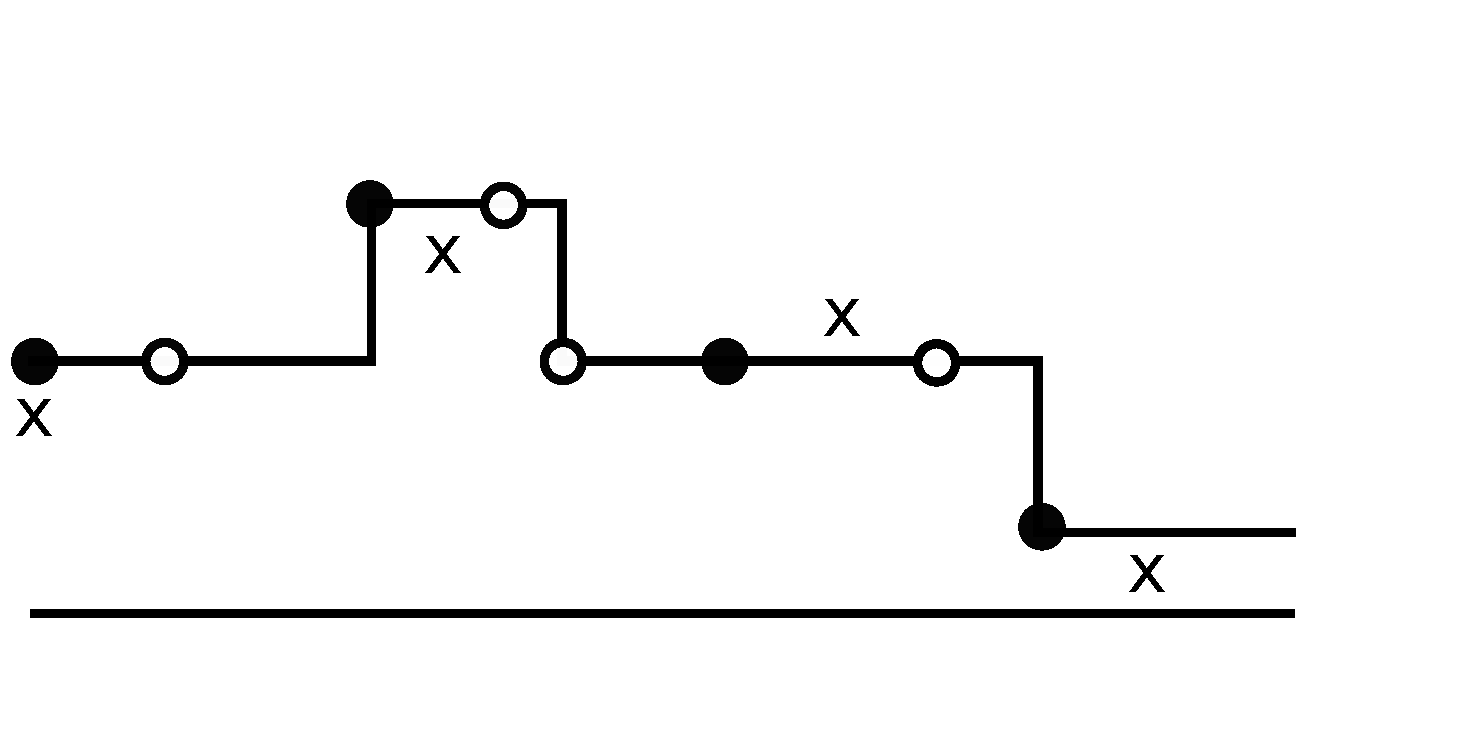
\includegraphics [width=0.64\textwidth, angle=0]{figs/VX.pdf}

  \end{minipage}
\caption{an example MJP path}
     \label{fig:vx}
  \end{figure}
{We recall some notation used in our proof. 
  The figure about shows a realization $S(t)$ of an MJP with rate matrix 
  $A(\theta)$ and initial distribution $\pi_0$ over an interval 
  $[0,t_{end}]$. The crosses are observations $X$. $\pi_0$ is the initial 
  distribution over states, and $\pi_\theta$ is the staionary distribution 
  of the MJP.
    $p(\theta)$ is the prior over $\theta$, and $q(\nu|\theta)$ is 
      the proposal distribution.
  \begin{itemize}
    \item The uniformized representation of $S(t)$ is the pair 
      $(V, W)$, with the Poisson grid 
      $W = [w_1, w_2, w_3, w_4, w_5, w_6, w_7]$ and the states 
      $V =[v_0, v_1, v_2, v_3, v_4, v_5, v_6, v_7]$ assigned with through 
      a Markov chain with initial distribution $\pi_0$ and transition 
      matrix $B(\theta,\theta')$. In the figure, the circles (filled and 
      empty) correspond to $W$.
    \item The more standard representation of $S(t)$ is the pair $(S,T)$.
      Here $T$ are the elements of $W$ which are true jump times (when 
      $V$ changes value), and $S$ are the corresponding elements of $V$.
      $U$ are the remaining elements of $W$ corresponding to self-transitions.
      Here, $T = [w_2, w_4, w_7]$ and $U = [w_1, w_3,  w_5, w_6]$. 
    \item The filled circles represent $W_X$, which are the elements of 
      $W$ containing observations. $V_X$ are the states corresponding to 
      $W_X$. In this example, $W_X = [w_2, w_5,w_7] \cup {\{0\}}$ and 
      $V_X = [v_2, v_5, v_7] \cup {\{v_0\}}$. 
    \item We write $\mW$ for the minimum number of elements of $W$ between 
      successive pairs of observations (including start time $0$). 
      In this example, $\mW = \min (3,3,2)= 2$. 
    \item $P(X | W, \theta, \theta')$ is the marginal distribution of 
      $X$ on $W$ under a Markov chain with 
      transition matrix $B(\theta, \theta')$ (after integrating out the 
      state information $V$). Recall that the LHS does not depend 
      on $\theta'$ because of uniformization.
    \item $P(X|\theta)$ is the marginal probability of the 
      observations under the rate-$A(\theta)$ MJP. 
$P(X | \theta) =  \int_W P(X | W, \theta, \theta') P(W|\theta, \theta')dW$.
    \item $P_B(V_X | W, \theta, \theta')$ is the probability 
      distribution over states $V_X$ for the Markov chain with 
      transition matrix $B(\theta, \theta')$ on the grid $W$, with the remaining elements 
      of $V$ integrated out. 
    \item  $P_{st}(V_X|\theta)$ is the probability of $V_X$ when 
      elements of $V_X$ are sampled i.i.d.\ from $\pi_\theta$).
    \item  $P_{st}(X|\theta)$ is the marginal probability of $X$
      when $V_X$ is drawn from $P_{st}(V_X|\theta)$.
  \end{itemize}
%\begin{align*}
%P(X | W, \theta, \theta') &= \sum_{V_X} P(X|V_X, \theta)P_B(V_X|W, \theta, \theta'),\\
%P_{st}(X | \theta) &= \sum_{V_X}P(X | V_X, \theta) P_{st}(V_X|\theta).
%\end{align*} 
} 
\setcounter{theorem}{3}

\subsection{Remaining proofs}
\begin{proposition}
The a posteriori probability that the embedded Markov chain makes a
self-transition,
$P(V_{i + 1} = V_i| W, X, \theta, \vartheta) \ge \delta_1 > 0$,
for %$i = 0, 1, 2, ..., |W|$ and
any $\theta,\vartheta, W$.
\end{proposition}
\begin{proof}
  We use $k_0$ from assumption~\ref{asmp:unif_rate}
  to bound {\em a priori} self-transition probabilities:
  \begin{align*}
    P(V_{i + 1}=s|V_i=s, W, \theta,\vartheta) &= B_{ss}(\theta,\vartheta) =
    1 - \frac{A_{s}(\theta)}{\Omega(\theta, \vartheta)}
    \ge 1 - \frac{A_{s}(\theta)}{\Omega(\theta)} \ge 1-\frac{1}{k_0}.
    \intertext{  We then have}
%\mathbb{E}[\mathbb{I}_{\{V_i = V_{i + 1}\}} | W, X, \theta, \theta^*]
  P(V_i = V_{i + 1} | W, X, \theta, \vartheta) &= \sum_v P(V_i = V_{i + 1}
  = v | W, X, \theta, \vartheta)
 =\sum_v \frac{P(V_i = V_{i + 1} = v, X | W, \theta, \vartheta)}{P(X | W,
 \theta, \vartheta)} \\
&=\sum_v \frac{P(X | V_i = V_{i + 1} = v, W, \theta, \vartheta)P( V_i =
V_{i + 1} = v|W, \theta, \vartheta)}{P(X | W, \theta, \vartheta)}\\
& \geq \frac{\lb}{\ub}\sum_v P(V_i = V_{i + 1} = v | W, \theta, \vartheta)\\
&=  \frac{\lb}{\ub} \sum_v P(V_{i + 1} = v | V_i = v, W, \theta,\vartheta)P(V_i = v | \theta, \vartheta) \\
& \geq \frac{\lb}{\ub} (1-\frac{1}{k_0}) \assign \delta_1 > 0.
\end{align*}
\qed
\end{proof}
\setcounter{theorem}{6}


\begin{proposition}
%Write $P(W', \theta' | W, \theta, \vartheta)$ for the transition kernel of our MCMC sampler given the observations. For any positive $\epsilon$, there exist $\theta_\epsilon > 0$ and corresponding $W_\epsilon > 0$, such that for any $\theta \ge \theta_\epsilon$, and any $\vartheta$, we have
  Let $(W, \theta, \vartheta)$ be the current state of the sampler.
 %Given this, let $E$ be the event that $| \alpha_I(\theta,\vartheta,X) -
 %\alpha(\theta,\vartheta,W',X)| \le \epsilon $.
%Write $q(W', \theta' | W, \theta, \vartheta)$ for the proposal
%distribution of our MCMC sampler.
Then, for any $\epsilon$, there exists $\theta_\epsilon > 0$ as well as a set $\E_\epsilon \subseteq \{(W', \theta'): |\alpha_I(\theta,\theta';X) - \alpha(\theta,\theta';W',X)| \le \epsilon\}$, such that for $\theta$ satisfying $\| \theta \| > \theta_\epsilon$ and any $\vartheta$, we have
%and $W_\epsilon > 0$, such that for
%$\theta \ge \theta_\epsilon$, and any $\vartheta$, we have
%  $P(|W'| > W_\epsilon, \theta' > \theta_\epsilon  | W, \theta, \vartheta) \ge 1-\epsilon$.
%  $| \alpha_I(\theta,\vartheta,X) - \alpha(\theta,\vartheta,W',X)|
%  \le \epsilon $ for any $(W', \theta')$ with $|W'| > W_\epsilon$ and $\theta' > \theta_\epsilon$.
  %$(\theta,\theta^*)$ satisfying
$P(E_\epsilon|W,\theta,\vartheta) > 1-\epsilon$.
\end{proposition}
\begin{proof}
  Fix $\epsilon > 0$ and $K > 1$ satisfying $(1 + \frac{1}{K})k_1 \ge 2$.
  \begin{itemize}
    \item  
From assumption \ref{asmp:prior}, there exist 
$M_\epsilon$ and $\theta_{1,\epsilon}$, such that 
$P(\frac{q(\theta | \theta')p(\theta')}{q(\theta' | \theta)p(\theta)}\leq M_\epsilon) > 1 - \epsilon / 2$ 
{for } $\theta$ satisfying $ \| \theta \| > \theta_{1,\epsilon}$.
    Define  $E_1^\epsilon = \{\theta' s.t.\ \frac{q(\theta | \theta')p(\theta')}{q(\theta' | \theta)p(\theta)}\leq M_\epsilon\}$.
    \item Define $E^K_2 = \{\theta' s.t.\ \frac{\Omega(\theta')}{\Omega(\theta)}\in [1/K, K] \}$.
Following assumption \ref{asmp:omega}, define $\theta_{2, \epsilon}^K$ 
such that $P(E^K_2 | \theta) > 1 - \epsilon / 2$ for all $\theta$ satisfying $\| \theta \| > \theta_{2, \epsilon}^K$.
    \item On the set $E^K_2$, $\Omega(\theta') \le K \Omega(\theta)$ (and also
$\Omega(\theta) \le K \Omega(\theta')$).  Lemma~\ref{lem:eigenvalue_lemma}
ensures that there exist $\theta_{3,\epsilon}^K > 0, w_\epsilon^K > 0$, 
such that for $\mW > w_\epsilon^K$, 
$ \| \theta \| > \theta_{3,\epsilon}^K$ and 
$ \| \theta' \| > \theta_{3,\epsilon}^K$, we have
$|P(X | W, \theta' , \theta) - P(X | \theta' )| < \epsilon$, and
$|P(X | W, \theta , \theta') - P(X | \theta )| < \epsilon$.
Define      $E_{3, \epsilon}^K = \{\theta' s.t. \| \theta'\| > {\theta}_{3,\epsilon}^K \}$.
    \item Define $E_{4, \epsilon}^K =\{W s.t.\ \mW >  {w}_{\epsilon}^K\}$.
Set $\theta_{4,\epsilon}^K$, so that for $\| \theta \| > \theta_{4,\epsilon}^K$, 
$ P(E_{4,\epsilon}^K|E^K_2, E_1^\epsilon ) > 1 - \epsilon.
%P(E_{4,\epsilon}^K | E_1^\epsilon E_2^K E_{3, \epsilon}^K) > 1 - \epsilon.
$. This holds since $W$ comes from a Poisson processes, whose rate can 
be made arbitrarily large by increasing $\Omega(\theta)$.
    \item From assumption \ref{asmp:mono_tail}, there exists $\theta_0$, such that $\Omega(\theta)$ increases as $\| \theta \|$ increases, for $\theta$ satisfying $\| \theta \| > \theta_0$.
Set ${\theta}_\epsilon =\max(\theta_0, \theta_{1, \epsilon},\theta_{2, \epsilon}^K,{\theta}_{3, \epsilon}^K, \theta_{4, \epsilon}^K)$. \\
  \end{itemize}
  Now consider the difference
\begin{align*}
|\alpha(\theta, \theta'; W, X) - \alpha_I(\theta, \theta'; X)| &= \ \mid 1 \wedge \frac{P(X | W, \theta' , \theta)q(\theta | \theta')p(\theta')}{P(X | W, \theta , \theta')q(\theta' | \theta)p(\theta)} - 1 \wedge \frac{P(X | \theta')q(\theta | \theta')p(\theta')}{P(X | \theta)q(\theta' | \theta)p(\theta)} \mid \\
& \leq \ \mid \frac{P(X | W, \theta' , \theta)}{P(X | W, \theta , \theta')} - \frac{P(X | \theta')}{P(X | \theta)}\mid  \frac{q(\theta | \theta')p(\theta')}{q(\theta' | \theta)p(\theta)}.
\end{align*}
%From assumption \ref{asmp:prior}, for any $\epsilon$, we can find a
%$\theta_{1,M}^\epsilon$  such that {for all } $\theta$ satisfying $ \| \theta \| > \theta_{1,M}^\epsilon$,
%\begin{align*}
%  P(E_1^\epsilon| \theta) > 1 - \epsilon / 2.
%\end{align*}
%the second term can be bounded with high probability. Also, given large $\theta$ and $\theta'$ which is close to $\theta$, the probability of $|W|$ being large is large.
%For $\epsilon / 4 > 0$,  from assumption \ref{asmp:prior}, there exists $\theta_2 > 0$ and $K_2 > 0$, such that for $\theta > \theta_2$, we have
%
%For $\epsilon/4 > 0$,
On $E^\epsilon_1$, $\frac{q(\theta | \theta')p(\theta')}{q(\theta' | \theta)p(\theta)} \le M_\epsilon$.
Since ${P(X | W, \theta , \theta')}$ and ${P(X | \theta)}$
are lower-bounded by $\lb$, for any $\epsilon > 0$ we can 
find a $K$ such that on $E^K_2 \cap E^K_{3,\epsilon}$,
%we can find a $\tilde{\theta}_{3,\epsilon}^K > 0, \tilde{w}_\epsilon^K > 0$ so that for $\mW > \tilde{w}_\epsilon^K$,
%$\theta$ satisfying $ \| \theta \| > \tilde{\theta}_{3,\epsilon}^K$ and $\theta'$ satisfying $ \| \theta' \| > \tilde{\theta}_{3,\epsilon}^K$, we have
\begin{align*}
|\frac{P(X | W, \theta' , \theta)}{P(X | W, \theta , \theta')} - 
   \frac{P(X | \theta')}{P(X | \theta)}| < \epsilon / M_\epsilon.
\end{align*}
This means that on $E^\epsilon_1 \cap E_2^K \cap E^K_{3,\epsilon}$,
$|\alpha(\theta, \theta', W, X) - \alpha_I(\theta, \theta', X)| < \epsilon$.\\
%For $\theta$ satisfying $ \| \theta \| > \kappa \tilde{\theta}_\epsilon$,where $\kappa > 1$ we have 
For $\theta > \max (\theta_{1,\epsilon},\theta^K_{2,\epsilon})$ 
%satisfying $ \| \theta \| > \kappa \tilde{\theta}_\epsilon$, where $\kappa > 1$ 
we have 
$
P(E^K_2 E^\epsilon_1) \ge P(E^K_2) + P(E_1^\epsilon) - 1 \ge 1 - \epsilon.
$\\
When $E^K_2$ holds, $\Omega(\theta') \ge \Omega(\theta)/K$.
For $\theta$ large enough, we can ensure $ \| \theta' \| > {\theta}^K_{3,\epsilon}$.
%with probability one, which means $P(E_{3,\epsilon}^K | E_2^K E_1^\epsilon) = 1$.\\
So \begin{align*}
P(E_1^\epsilon E_2^K E_{3,\epsilon}^K E_{4,\epsilon}^K) > (1- \epsilon)^2.
\end{align*} 
Finally, set $E_\epsilon \assign E_1^\epsilon \cap E_2^K \cap E_{3,\epsilon}^K \cap E_{4,\epsilon}^K$ , giving us our result.

% Call this event $E_{3,K}^\epsilon$. Necessary for $E_3^{K}$ given $E_2^{K}$ is that
% $\mW > W^K_3$ for our choice of $K$. As before, we can find a $\theta_{4,\epsilon}$
% such that for $\theta$ satisfying $ \| \theta \|  > \theta_{4,\epsilon}$, this probability can brought arbitrarily close to $1$.
% %For the $W_4$, there exists $\theta_5 > 0$, such that for $\theta > \theta_5$, and any $\theta'$ with $\frac{1}{K_3}  \leq \frac{\Omega(\theta')}{\Omega(\theta)}  \leq K_3$, we have \begin{align*}
% %P(|W'| > W_4 | W, \theta, \theta', \vartheta) > 1- \epsilon / 4.
% %\end{align*}

% %\{
% %There exists $\theta_6 > 0$, such that for $\theta > \theta_6$, we have
% %\begin{align*}
% %P(\theta' > \theta_4 | \theta) > 1 - \epsilon / 4.
% %\end{align*}}

% %So given the current state $(W, \theta)$, and $K_0$, $P(\{ \frac{1}{K_0}\leq \frac{\Omega(\theta')}{\Omega(\theta)} \leq K_0 \} \cap \{ \frac{q(\theta | \theta')p(\theta')}{q(\theta' | \theta)p(\theta)} \leq 2\}| \theta ) > 1 - 2\epsilon / 4 $, for any $\theta > \max(\theta_2, \theta_3)$.\\

% Given current state $(W, \theta)$, set $\theta_\epsilon =
% \kappa \max(\theta_{1, M}^\epsilon,\theta^K_{2, \epsilon},\theta^K_{3, \epsilon}, \theta_4)$, $\kappa > 1$.
% %$E_1 = \{ \frac{q(\theta | \theta')p(\theta')}{q(\theta' | \theta)p(\theta)} \leq \max(K_2, 1) \}$ and
% %$E_2 = \{ \frac{\Omega(\theta')}{\Omega(\theta)}  \leq K_3\}$.
% For $\theta$ satisfying $ \| \theta \| > \theta_\epsilon$, $P(E^K_2 | E_1)>1-\epsilon$, and
% \begin{align*}
% P(E_1E^K_2) %&= P(E_1) + P(E_2) - P(E_1 \cup E_2) \\
% & = P(E_1) P(E^K_2|E_1) \ge (1 - \epsilon)^2.
% \end{align*}
% When $E^K_2$ holds, $\theta' \ge \Omega^{-1}(\Omega(\kappa\theta)/K)$.
% By choosing $\kappa$ large enough, $\theta'$ satisfying $ \| \theta \| > \theta^K_3$. Then, for
% $E_3$ to hold, we only need $|W| > W^K_3$. This holds with probability
% greater than $1-\epsilon$, so that
% \begin{align*}
%   P(E_1E_2E_3) > (1- \epsilon)^3.
% \end{align*}
% Finally, let $E_\epsilon \assign E_1\cap E_2 \cap E_3$ , giving us our result.
% %with probability greater than $1 - \epsilon$.

% %Also, the set
% %For $K = 1$ and $\epsilon$, there exists $\theta_1$ such that for $\theta > \theta_1$, $\mid \frac{q(\theta | \theta')p(\theta')}{q(\theta' | \theta)p(\theta)}\mid \leq 1$ with probability close to 1. Given $\theta$ and $\theta'$, $P(|W'| > W_0 | \theta, \theta')$ is close to 1.

\end{proof}
